% 中点四边形 例2：矩形 -> 中点四边形是菱形
\documentclass[tikz,border=4pt]{standalone}
\usepackage{ctex}
\usepackage{amsmath}
\usetikzlibrary{calc}
\begin{document}
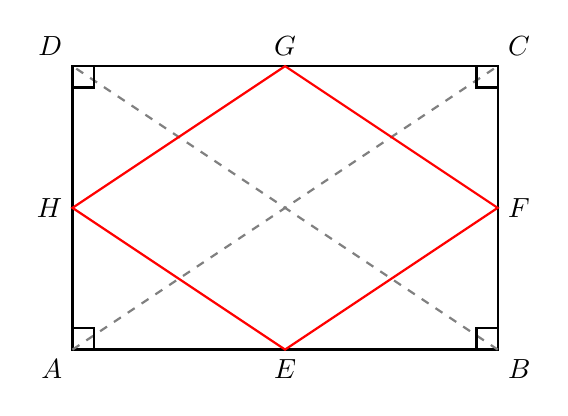
\begin{tikzpicture}[scale=0.9, thick]
  \coordinate (A) at (0,0);
  \coordinate (B) at (6,0);
  \coordinate (C) at (6,4);
  \coordinate (D) at (0,4);
  \coordinate (E) at (3,0);
  \coordinate (F) at (6,2);
  \coordinate (G) at (3,4);
  \coordinate (H) at (0,2);
  \draw (A)--(B)--(C)--(D)--cycle;
  \draw[gray, dashed] (A)--(C);
  \draw[gray, dashed] (B)--(D);
  \draw[red] (E)--(F)--(G)--(H)--cycle;
  % 直角小方块
  \foreach \pt/\a/\b in {A/0/90, B/90/180, C/180/270, D/270/0}{
    \draw ($(\pt)+({0.3*cos(\a)},{0.3*sin(\a)})$)
          -- ($(\pt)+({0.3*cos(\a)+0.3*cos(\b)},{0.3*sin(\a)+0.3*sin(\b)})$)
          -- ($(\pt)+({0.3*cos(\b)},{0.3*sin(\b)})$);
  }
  \node[below left] at (A) {$A$};
  \node[below right] at (B) {$B$};
  \node[above right] at (C) {$C$};
  \node[above left] at (D) {$D$};
  \node[below] at (E) {$E$};
  \node[right] at (F) {$F$};
  \node[above] at (G) {$G$};
  \node[left] at (H) {$H$};
\end{tikzpicture}
\end{document}
